%\subsection{UCW9 - Modifica parametri di ordinamento classifica}
\begin{figure}[!h]
\centering
    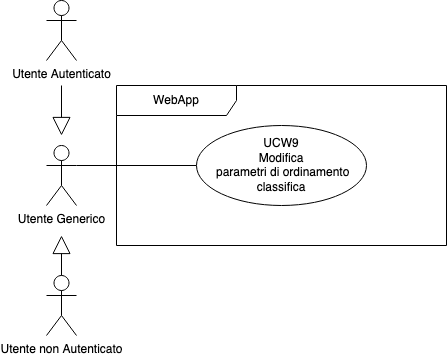
\includegraphics[scale=0.5]{UC_images/UCW9.png}
    \caption{UCW9 - Modifica parametri di ordinamento classifica}
\end{figure}
\begin{itemize}
	\item \textbf{Descrizione}: L'utente generico modifica i parametri di ordinamento della classifica con i risultati dei locali.
    \item \textbf{Attore primario}: Utente generico.
    \item \textbf{Precondizione}: L’utente sta visualizzando la classifica (UCW7 §3.8).
    \item \textbf{Postcondizione}: L’utente visualizza a schermo la classifica dei migliori locali gastronomici riordinata in base ai parametri di ordinamento inseriti.
    \item \textbf{Scenario principale}: 
    \begin{enumerate}
        \item L’utente clicca il pulsante “modifica parametri di ordinamento”;
        \item L’utente modifica i parametri di ordinamento;
        \item L’utente clicca il pulsante “applica parametri”.
    \end{enumerate}

    \item \textbf{Sottocasi}:
    \begin{enumerate}
        \item Modifica peso dei social (UCW9.1 §3.10.1);
        \item Modifica peso dei tipi di contenuto (UCW9.2 §3.10.2).
    \end{enumerate}

\end{itemize}

\begin{figure}[!h]
\centering
    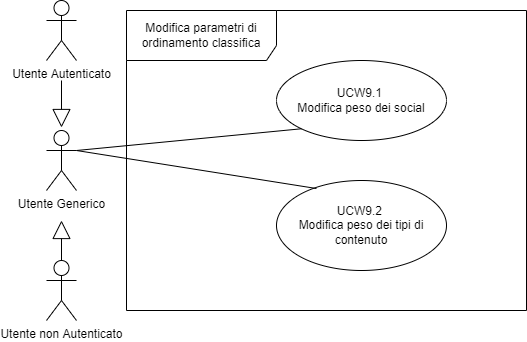
\includegraphics[scale=0.5]{UC_images/UCW9-.png}
    \caption{Sottocasi UCW9}
\end{figure}

\subsubsection{UCW9.1 - Modifica peso dei social }
\begin{itemize}
	\item \textbf{Descrizione}: L'utente generico modifica l'ordinamento della classifica in base al peso dei social.
    \item \textbf{Attore primario}: Utente generico.
    \item \textbf{Precondizione}: L’utente sta visualizzando la classifica (UCW7 §3.8) e ha premuto il pulsante “Modifica Parametri di Ordinamento”.
    \item \textbf{Postcondizione}: Il parametro in questione viene applicato.
    \item \textbf{Scenario principale}: 
    \begin{enumerate}
        \item L’utente modifica il peso in percentuale che forniscono i contenuti di ciascun social tramite una barra percentuale;
        \item L’utente clicca il pulsante “OK”.
    \end{enumerate}
\end{itemize}

\subsubsection{UCW9.2 - Modifica peso dei tipi di contenuto}
\begin{itemize}
	\item \textbf{Descrizione}: L'utente generico modifica l'ordinamento della classifica in base al peso dei tipi di contenuto.
    \item \textbf{Attore primario}: Utente generico.
    \item \textbf{Precondizione}: L’utente sta visualizzando la classifica (UCW7 §3.8) e ha premuto il pulsante “modifica parametri di ordinamento”.
    \item \textbf{Postcondizione}: Il parametro in questione viene applicato.
    \item \textbf{Scenario principale}: 
    \begin{enumerate}
        \item L’utente modifica il peso in percentuale che forniscono i tipi di contenuto (foto, post, stories, commenti) tramite una barra percentuale;
        \item L’utente clicca il pulsante “OK”.
    \end{enumerate}
\end{itemize}

\pagebreak